\section{Requisitos}
Este proyecto tiene como objetivo crear una plataforma donde por un lado los
usuarios vulnerables de la carretera (\gls{vru}), formados por los ciclistas, y
por el otro lado los vehículos se comuniquen con un sistema central que se
encargue de detectar situaciones de peligro entre ellos y los avise cuando esto
pueda suceder. Tras obtener una descripción completa del proyecto, se han
realizado varias reuniones en las cuales se han definido las especificaciones.
Durante la fase inicial del proyecto se han recogido los requisitos funcionales
y se han priorizado de la siguiente manera:

\begin{enumerate}
	\item Empleo de comunicaciones \Gls{802.11p} (mediante los módulos de NEC) y
	redes móviles entre dispositivos móviles.
	\item Debe ser una comunicación bidireccional.
	\item Baja latencia en el envío de mensajes; menor a 100 ms.
	\item Incremento de la seguridad para los \gls{vru}.
	\item Comunicación de ciclistas individuales y en grupo.
	\item Se debe conocer la posición de los ciclistas en los vehículos a motor,
	y recibir avisos.
\end{enumerate}

Se han clasificado las siguientes especificaciones como requisitos ni
funcionales, ya que no son vitales para el despliegue principal de la plataforma,
pero que pueden ser integrados tras el despliegue inicial:
\begin{itemize}
	\item Aplicación con monitor de actividad para ciclistas.
	\item Posibilidad de crear logs durante las pruebas.
	\item Simpleza al crear un grupo de ciclistas, que no requiera conocimientos
	técnicos.
	\item Posibilidad de mandar mensajes desde el servidor central.
\end{itemize}

En el diagrama \ref{fig:casos_de_uso} se pueden observar las tareas que se han
pedido integrar en el proyecto: los ciclistas envían sus posiciones al iniciar
la salida, pueden crear un grupo o no, monitorizar su actividad y emparejar sus
dispositivos con el casco \gls{ble}. Los conductores al iniciar su aplicación
son notificados sobre los eventos de alerta que se pueden dar en la carretera,
mientras en segundo plano notifican su posición. La plataforma que es
implementada en la nube recibe las notificaciones y cuando detecte alguna
posibilidad de peligro, notifica a los ciclistas y conductores. Además, desde la
aplicación de escritorio en la nube se pueden enviar mensajes para la gestión de
tráfico a la \gls{rsu}.

\begin{figure}[H]
	\begin{center}
		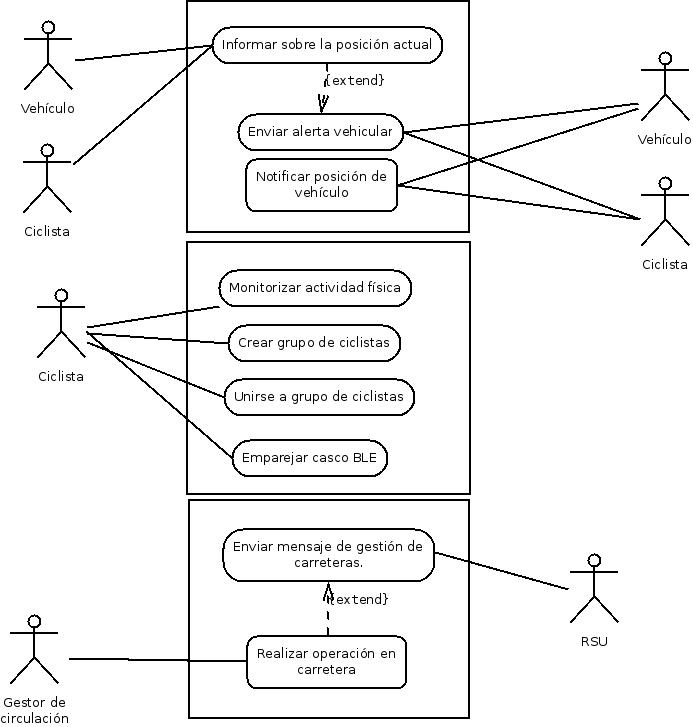
\includegraphics[scale=0.4]{casos_de_uso}
		\caption{Casos de uso}
		\label{fig:casos_de_uso}
	\end{center}
\end{figure}

Una vez analizados los requisitos de la plataforma, se procede a diseñar la
solución del sistema. Una primera decisión que se debe tomar es si el sistema
debe ser distribuido o centralizado. El primero tiene la ventaja de proveer un
mejor rendimiento, ya que tan solo debe encargarse de un área, pero puede perder
información ya que no tiene un mapa completo del área total. Por el contrario,
un sistema centralizado requiere de una mayor infraestructura cuanto más área
provea de cobertura, pero tiene en todo momento una visión completa de los
escenarios. Al ser una solución experimental que va a ser desplegada en un
pequeño escenario y los requisitos de seguridad son prioritarios, se ha elegido
un sistema centralizado.

Se deberá crear diferentes aplicaciones: un servidor central que permita la
comunicación entre diferentes tecnologías, una aplicación móvil para ciclistas y
conductores, y aplicaciones para ser desplegadas en unidades \gls{obu} y
\gls{rsu}.
